%2345678901234567890123456789012345678901234567890123456789012345678901234567890
%%%%%%%%%%%%%%%%%%%%%%%%%%%%%%%%%%%%%%%%%%%%%%%%%%%%%%%%%%%%%%%%%%%%%%%%%%%%%%%%
% MAURICIO ESGUERRA NEIRA
% Ph. D. Thesis
%%%%%%%%%%%%%%%%%%%%%%%%%%%%%%%%%%%%%%%%%%%%%%%%%%%%%%%%%%%%%%%%%%%%%%%%%%%%%%%%
\chapter{Introduction}
\label{introduction} 
\bibliographystyle{nar}
\section{RNA folding}
The first  high resolution X-ray\index{X-ray} structure  of RNA larger
than a dinucleotide was  that of yeast tRNA$^{\textrm{Phe}}$ at 3{\AA}
in 1974 \cite{robertus1974, kim1974}. Thirtysix years later there are two
orders of magnitude more RNA structural information \cite{noller2005},
and new  information from non-coding RNA's is  expected \cite{weinberg2009}.  This  fact and
the discovery  of ribozymes \cite{kruger1982,  takada1983} has renewed
interest in  solving the RNA folding\index{RNA  folding} problem, that
is, from  primary sequence, finding in  an automated\footnote{The term
  automated  is used  here to  mean  a theoretical  model of  tertiary
  folding,  which   could  use  experimental   measures  of  secondary
  structure association in the same way that the traditional secondary
  structure  folding  model  \cite{zuker1989, hofacker1994}  uses  the
  Tinoco-Uhlenbeck  dinucleotide  postulate  \cite{borer1974} to  find
  total free energies.} way  the native three-dimensional structure of
RNA  and  its  folding  pathway. The  RNA  folding\index{RNA  folding}
problem is usually  seen as analogous to the  protein folding problem,
due  both  to   the  discovery  of  the  enzymatic   behavior  of  RNA
\cite{kruger1982, takada1983} and the complicated folding of large RNA
molecules  \cite{batey1999}.  To  take  advantage of  this analogy,  a
unified conceptual  framework for describing RNA  and protein folding,
called the kinetic partitioning mechanism (KPM), has been developed by
Thirumalai and Hyeon \cite{thirumalai2005}. This and other methods are
based on  defining an adequate  partition function for  describing the
correct  conformational  ensemble  of  folded, partially  folded,  and
unfolded  structures   \cite{chen1995,  chen1998,  thirumalai1996}  of
either protein or RNA.

\section{Is RNA folding a hard or easy problem?}
There are two trains of thought regarding RNA folding. One states that
RNA  folding is  less complex  than protein  folding \cite{tinoco1999}
because RNA is made up of a four letter alphabet of similar nucleotide
units   instead  of  a   20  letter   alphabet  of   dissimilar  amino
acids.  Therefore the  number of  possible sequential  combinations is
smaller.  It   is  also  well   known  that  secondary   and  tertiary
interactions can  be separated in  the case of  RNA by the  absence or
presence  of  Mg$^{2+}$ \cite{rangan2003}  (see  Figure 1.1),  whereas
secondary  and  tertiary  elements  are  not as  easily  separable  in
proteins.
\begin{figure}[ht]
\centering
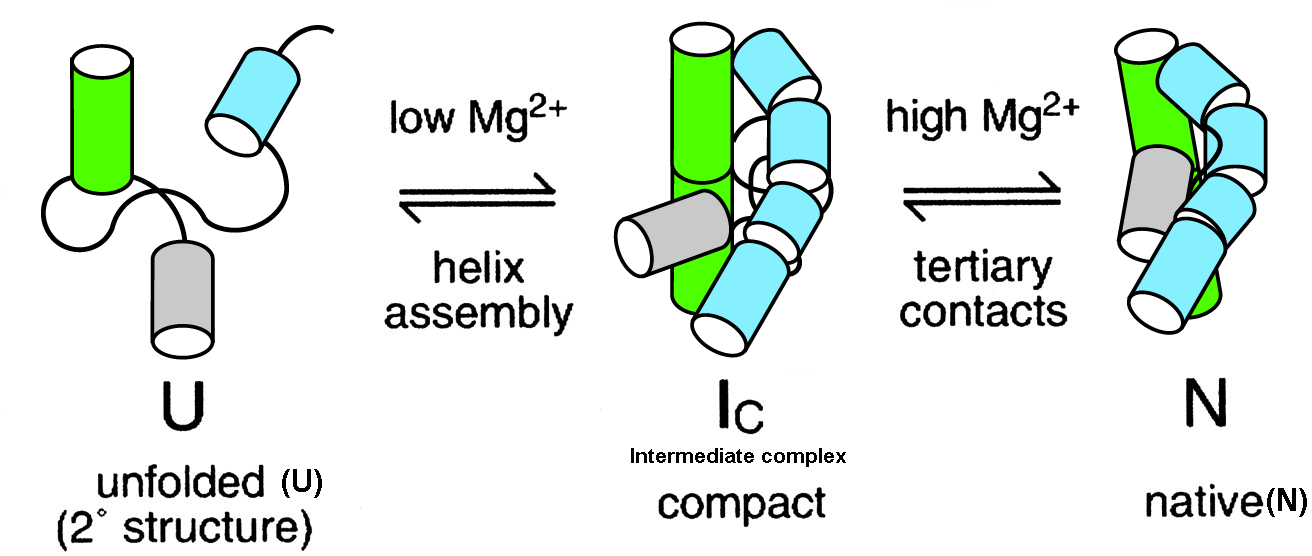
\includegraphics[scale=0.3]{Chapter1/rangan2003pnas.png}
\caption{Separation of secondary and tertiary interaction in
RNA \cite{rangan2003}. Double helical secondary structure
represented  by individual cylinders and tertiary interactions by
association of cylinders.}
\end{figure}
The  other point of  view says  that RNA  folding can  be at  least as
complex as protein folding \cite{moore1999a, sorin2004} since there is
no such thing  as hydrophobic burial of regions of RNA  as in the case
of proteins.  Instead, the electrostatic  problem of having  a complex
charged backbone must be dealt with in the case of RNA.
% The case of the electrostatic treatment of the backbone is lacking
% here, most likely WKO wants me not to ignore our own Gerald Manning
% tinoco 1999 says this must be an easy to solve problem since we can
% do the electrostatics for it easily
For instance,  the interactions of  the RNA polyanionic  backbone with
water  and cations  \cite{klein2004a}  are not  easily simulated  with
explicit   solvent  models   as  can   be  done   for   proteins.  The
aforementioned interactions of RNA  need to be modeled implicitly, and
must aim to describe long dynamic processes of the order of seconds to
minutes,  in  contrast   to  the  typical  time  scales   of  tens  of
microseconds associated with protein folding.
% Remember that this means that a explicit calculation for RNA would
% be prohibitively large.
Although   secondary   and  tertiary   structure   can  be   separated
experimentally, there have been few theoretical efforts to account for
the  folding  of  RNA  from  a random  sequence  of  nucleotides  into
secondary structures and tertiary  structures. What little is know has
been  investigated at  low  resolution. Professor  Stephen Harvey  and
associates     have     simulated     yeast     tRNA$^{\textrm{Phe}}$,
\cite{malhotra1990}  and  the  assembly  of  the 30S  subunit  of  the
ribosome \cite{stagg2003} at various levels of detail, initially using
only one pseudoatom  per helical region, and later  one pseudoatom per
nucleotide. Recently Major's group \cite{parisien2008} at Montreal has
proposed a  pipeline of two  computer algorithms, one  makes secondary
structure predictions, and the  other assembles 3D structures based on
the best scoring  secondary structures. The key to  the success of the
3D prediction is attributed to what they call Nucleotide Cyclic Motifs
(NCM), which  are based on  a graph theoretical description  common to
secondary and 3D structure.
% Note for presentation ==> Include figure 1 in Malhotra-harvey paper
% Look at what says in folding.stanford.edu/science.html Also take
% into account Biophys J. V.88 2516-2524 for the case of having to
% think of water in the folding problem.
By contrast,  in the case of  proteins many groups  have simulated the
transition  from  secondary  to  tertiary  structure,  including  some
calculations which  account for the  strong coupling of  secondary and
tertiary  structure   \cite{westhead1999,  gerstein2003,  meiler2003}.
This type of work is  often referred to as protein structural topology
and there is no counterpart for RNA.

%The seminal paper here seems to be the one of liphardt in 2001 for
%rna unfolding
\section{Experimental folding techniques}
Traditionally   RNA   folding  and   unfolding   have  been   followed
calorimetrically  and spectroscopically as  a function  of temperature
and  cation concentration  \cite{bloomfield2000}. While  this approach
works well  for studying two-state  folders, \textit{i.e.}, structures
which populate only  two states (native and melted),  in general RNA's
are  not two-state  folders. RNA  seems to  go through  a  rugged free
energy  landscape   of  conformations   in  the  process   of  folding
\cite{zhuang2003}.  The  experimental  solution  to  this  problem  is
offered  by  single molecule  techniques  like fluorescence  resonance
energy transfer (FRET) and  mechanical micromanipulation, in which the
ends of RNA  are attached to micron sized beads  which are then pulled
apart  and  monitored  with  a laser  light  trap  \cite{liphardt2001,
  onoa2004,  tinoco2004, hyeon2005}.  In the  case of  single molecule
force-induced   unfolding,  state   transitions   often  occur   under
non-equilibrium  conditions, thereby  making it  difficult  to extract
equilibrium  information from the  data. Recently  Bustamante, Tinoco,
and associates  have shown that  using the Crooks  fluctuation theorem
\cite{crooks1999},  one  can deal  with  such  cases  and extract  RNA
folding    free   energies    from    single   molecule    experiments
\cite{collin2005}.
%\subsection{RNA Folding in Vitro vs in Vivo vs in Silico}
% It still is to be seen whether the following is relevant or not
% This single molecule information is
% collected in-vitro and not in-vivo, which is actually the ultimate
% problem aimed for prediction, there's quite a lot of evidence for
% different folding states reached in one case and not the other and
% viceversa \cite{sosnick2003, schroeder2002} but still a first step
% towards understanding in-vivo folding is in-vitro and in-silico
% experimentation.

\section{RNA simulations}
Network  and molecular  mechanics-molecular  dynamics (MM-MD)  methods
provide  useful  information  relevant  to the  RNA  folding-unfolding
problem, especially  for describing fluctuations away  from the native
conformation.  Gaussian  network  models \cite{y_wang2004,  bahar1998,
  wang2005} which treat RNA at  less than atomic detail have been used
to describe  the motions  of large RNA  structures like  the ribosome.
Examples of the  predicted normal modes of motion  of the ribosome can
be  seen  at:  http://ribosome.bb.iastate.edu/70SnK  mode.  Using  MM,
Sanbonmatsu and  coworkers obtained a  static atomic model of  the 70S
ribosome structure through homology modeling \cite{tung2004}. Tung and
associates used  this structure for  an all-atom MD simulation  of the
movement of  tRNA into a  fluctuating ribosome \cite{sanbonmatsu2005}.
This type of simulation might  be useful in a reverse-folding approach
to  the  RNA folding  problem.  To the  best  of  our knowledge,  such
calculations haven't as yet been done for RNA.

\subsection{Local nucleotide interactions}
%\subsubsection{QM approaches and MM consequences}
The molecular  interactions which rule  RNA structures at  the nucleic
acid base level, \textit{i.e.},  local level, are hydrogen bonding and
stacking interactions. The former are  related to base pairing and the
latter, in most cases, to  nucleotide steps. These interactions can be
explored  theoretically at various  levels. At  the highest  level are
ab-initio  quantum   mechanical  calculations  which   are  still  too
expensive   for  systems  as   large  as   hundreds  of   atoms.  Such
calculations,  nevertheless,  can  tell   a  great  deal  about  local
electronic behavior.  For example, Hobza and  collaborators have found
that the  stacking interaction of free nucleotide  bases is determined
by   dispersion  attraction,   short-range  exchange   repulsion,  and
electrostatic  interaction.  No  specific $\pi-\pi$  interactions  are
found     from    electron    correlated     ab-initio    calculations
\cite{sponer1996, sponer1997}.  This is  why force field  methods have
been so successful in the  study of nucleic acids, since the empirical
potentials used  in such studies  mimic well the  quantum mechanically
obtained energy profiles \cite{tung2004, sponer2000}.
% since they can be modeled easily with simple empirical potentials
% consisting of Lennard-Jones, van der Waals and Coulomb terms.
% What the recent results say it's simply that by using a larger
% basis set, they can account for some interactions which were not
% included before, and maybe because of taking better account of
% electron-correlation.
A currently debated ab-initio finding is whether small fluctuations in
the   configurations   of   neighboring   base  pairs   (dimers)   are
iso-energetic  or  not.  Recent   calculations  of  Sponer  and  Hobza
\cite{sponer2006}   seem  to   contradict  their   older  publications
\cite{sponer2000,  hobza2002},  in which  the  stacking energies  were
reported to  be relatively insensitive to dimer  conformation. The new
results  use  the so-called  ``coupled  cluster  singles doubles  with
triple electron excitations'' CCSD(T)  method, to account for electron
correlation.  Using  this electron correlation  energy correction, the
stacking energy differences between dimer conformations turn out to be
considerably higher than previously reported.

% therefore justifying rigid body parameter interpretations.
% \subsubsection{Experimental Stacking and Polyionic backbone}
Single  and  double strand  stacking  free  energies  can be  obtained
calorimetrically.  The most  popular  method used  for obtaining  such
quantities     is    differential    scanning     calorimetry    (DSC)
\cite{marky1982}.  These   measurements  show  favorable  dinucleotide
stacking free  energies as  large as -3.6  kcal/mol for  double strand
stacking.  Experimentally, the  magnitudes of  these  interactions are
found  to be  sequence dependent  \cite{bloomfield2000}. In  fact, the
stacking free  energies for some  sequences\footnote{Unpaired terminal
  nucleotides UC/A UU/A at 1M  NaCl.} are found to be negligible. Thus
there  may be  no accountable  stacking  interaction at  all for  some
sequences.

Besides  taking into  account  the effects  of  stacking and  hydrogen
bonding,  it  is  important  to  think  at the  same  time  about  the
polyelectrolyte  nature  of  the  RNA backbone.  Manning's  counterion
condensation theory \cite{manning1977,  manning2003} provides a simple
and  quantitative picture of  the interactions  of the  double helical
nucleic acid polyanion with its counterions, although it does not take
into account  the discrete  nature of charge  \cite{bloomfield2000} or
the folding  of RNA. Poisson-Boltzmann  theory offers a  more detailed
picture   of   the  behavior   of   charged   macroions  in   solution
\cite{antypov2005}.
% Talk more about counterion condensation, thirumalai discusses it on
% his 2001 paper also chapter 8 of Bloomfield, Crothers, Tinoco
% (References \cite{manning2003} Ray-Manning?).
% Real Experiments results for stacking energies and polyanion
% energies and Energetics related to cation metal presence
% WKO says that there might be old experimental data that are contrary
% to this and that I must show it here, so far what I've found is
% Saenger saying that based on old QC and this is different, he
% relates it to hydrophobicity concepts. Talk about experiments.

The local conformational  space of RNA has been  studied using a large
set of available  RNA structures from the Nucleic  Acid Database (NDB)
\cite{berman1992}.  The torsion  angles of  the nucleotide  steps have
been  clustered  in the  parameter  space  using different  techniques
\cite{murray2003,  schneider2004}.   The  root-mean-square  deviations
(RMSD)  of   the  distances  between  closely  spaced   atoms  in  the
phosphates,   sugars,   and    bases,   have   also   been   clustered
\cite{sykes2005}. The  latter studies are aimed at  finding the common
nucleotide base  steps and base-pair  building blocks which  are given
the name of RNA doublets.  Recently, the RNA Ontology Consortium (ROC)
has  proposed   a  consensus   set  of  RNA   dinucleotide  conformers
integrating the work of various groups \cite{richardson2008}.


\subsection{RNA secondary structure algorithms and the lack of
tertiary  ones} From  secondary structure  prediction  algorithms like
Zuker's \textit{mfold} program \cite{zuker2003}, Hofacker's Vienna RNA
package  \cite{hofacker1994}, or Mathews  Dynaling \cite{mathews2002},
one  obtains a large  ensemble of  secondary structure  graphs.  These
graphs  can be  analyzed  with  graph theory  to  produce a  partition
function  describing a  full  arrangement of  contacts  for the  total
number of possible secondary structures making possible a "relation of
microscopic      conformations     to      macroscopic     properties"
\cite{chen2000}. So far this type of model has not been generalized to
take  into   account  tertiary  structural   features,  \textit{i.e.},
interhelical interactions of RNA.
In the  last two to  three years a
boom  in  prediction  of  small  ($\approx$  200  nucleotides)  RNA  3D
structures has started. Basically  three types of approaches are being
followed.  One is that  of using  a coarse  grained model  assigning a
potential function  to it, followed  by a minimization  procedure, and
then  a molecular  mechanics (MM)  all atom  refinement \cite{das2007,
  ding2008,  jonikas2009a}. Another  starts  from predicted  secondary
structures  and  assumes  their   helical  regions  adopt  the  A-form
conformation, then mechanically thrusts residues as rigid bodies in the
remaining non-helical regions, and finally carry out an MM optimization
\cite{martinez2008}.  Finally,  a pipeline between  secondary structure
prediction, and tertiary structure assembly is proposed. This pipeline
uses  as  bridging concept  between  2D  and  3D structure  the  graph
theoretical concept  of a minimal cycle  basis, which for  the case of
nucleic acids they rename as Nucleic Cyclic Motifs (NCM) \cite{parisien2008}.

\subsection{RNA overall fold}
Whereas in the case of proteins one can describe the overall fold from
the  arrangement of secondary  structure motifs,  \textit{i.e.}, using
the   helix-ribbon-coil   images    developed   by   Jane   Richardson
\cite{richardson2000} (see  Figure 1.2), there is  still no comparable
description of the overall fold of RNA. A ribbon representation of the
sugar  phosphate backbone  helps to  understand the  folding  of small
RNA's, but in the case of  the ribosome this type of representation is
not sufficient, see Figure 1.3.

\begin{figure}[ht]
\centering
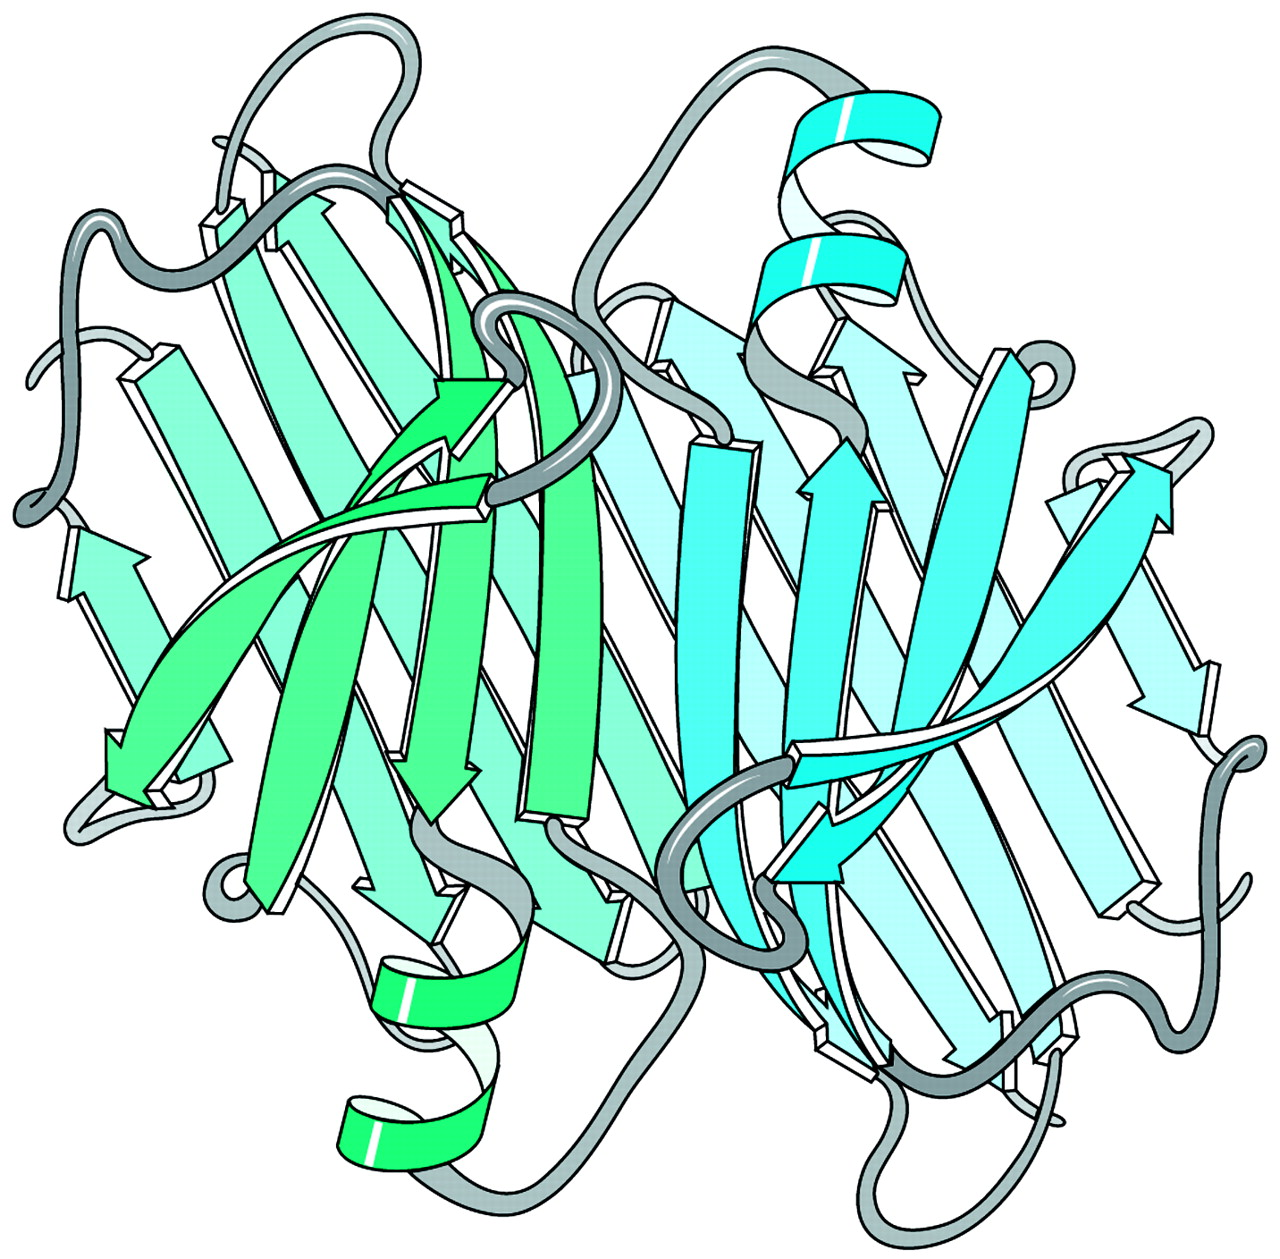
\includegraphics[scale=0.4]{Chapter1/overallfold.png}
\caption{Ribbon-coil schematic illustraring the fold and
  intermolecular units of a dimer of prealbumin, or
transthyretin, taken from Richardson \textit{et al.} \cite{richardson2002}}
\end{figure}

\begin{figure}[t]
\centering
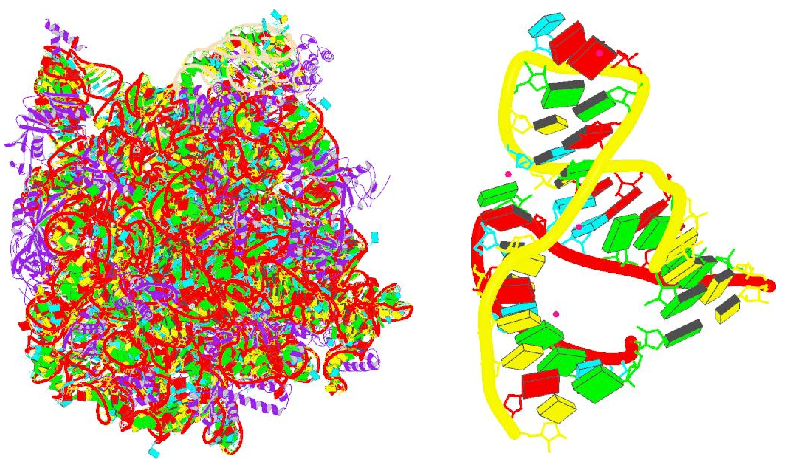
\includegraphics[scale=0.5]{Chapter1/ribosome_ribozyme.png}
\caption{\textit{Haloharcula marismortui's} large ribosomal subunit
(left) and hammerhead ribozyme (right).%NDBID:UR0029
 The figures were taken
directly from the NDB web pages, and show a ribbon
representation of the phosphate backbone, and a block representation
for the nucleotide bases. From the figures it's clear that, whereas the
ribozyme fold can be clearly understood with this representation, the
ribosome fold cannot.}
\end{figure}

One can envision that a  thorough investigation of the parameter space
of  translational and  rotational degrees  of freedom  of  the helical
regions of RNA could give clues as to how we might see an overall fold
in RNA structures.

In  the  case  of  proteins  the SCOP  (Structural  Classification  of
Proteins)  database  \cite{andreeva2004},  classifies proteins,  among
other   classifications,  according   to  recurrent   arrangements  of
secondary   structure,   that   is,   folds.  The   SCOR   (Structural
Classification of RNA) database \cite{klosterman2002, klosterman2004},
aims  to  provide  a  similar  classification  to  that  obtained  for
proteins,   but   using   RNA  motifs\footnote{Leontis   and   Westhof
  \cite{leontis2003}  define  RNA  motifs  as: "Directed  and  ordered
  arrays  of  non-WC  (Watson-Crick)  base-pairs  forming  distinctive
  foldings  of the  phosphodiester  backbones of  the interacting  RNA
  strands"} instead. This classification  focuses on the local folding
of small pieces of RNA and cannot describe the overall fold.

\subsection{RNA motifs}
The current review on RNA motifs spans (mainly) the first decade of the
XXI century. It is arranged in chronological order from the date of the
most recent publication to the oldest one. The header indicates the group
leader and current location.\\

- \textbf{SCHLICK GROUP at NYU.}\\
Analysis of four-way junctions and higher order junctions.
Using Leontis group software, FR3D, junctions of order four or higher are found
and then are classified according to whether they form coaxial stacks
or not, and so on. It seems like most of the analysis is based on
visual inspection. (2009)
\cite{laing2009} \cite{laing2009a}\\

- \textbf{LEONTIS GROUP at Bowling Green U.}\\
Book chapter which brings together many of Leontis papers into the
software named FR3D, which unfortunately is coded in matlab and makes a
GUI windows executable which is very hard to adapt to efficient
analysis of many structures through command line scripts. They also
provide new definitions for RNA motifs extending the vocabulary for
naming them, that is, they start using terms such as ``\textit{3D structural
RNA motifs}'', and ``\textit{modular RNA 3D motifs}'', to further
distinguish them from sequence alone motifs, or from secondary structure
motifs. Another new contribution is to explicitly show examples where
sequences of different length form the same motif, as is the case with
the GNRA loop. Finally, for differentiating between functional motifs,
and structural motifs they show the example of the 23S subunit of rRNA
for two different species, where in one case part of a helix is
smaller than in the other, but nonetheless the geometry is the same
where helices 63 and 101 are contacting each other, therefore
presenting a somewhat self-contradictory statement since the final
emphasis is put into the three dimensional configuration (structure
determining function) which is retained. (2009)
\cite{nasalean2009}\\

- \textbf{SCHROEDER GROUP at Oklahoma U.}\\
Gives an up to date description of the main programs and algorithms
used for RNA secondary structure prediction. The article focuses on
the major groups, i.e., Turner-Mathews, Zucker, Hofacker-Stadler,
Major, and it also gives the location of their software and a good
list of online tools. (2009)
\cite{schroeder2009}\\

- \textbf{FRENKEL GROUP at UCSF.}\\
ISfold is a matlab program for examination of patterns of nucleotide substitutions
from  sequence   alignments  or  mutation  experiments.  It can
identify plausible base  pair interactions. It Identifies the
existence of non-WC base pairs within RNA  bulges, internal  loops,
and hairpin  loops, structures that cannot be easily
predicted   with   existing algorithms. The IS in ISfold stands for
iso-steric in the same sense as isostericity is treated by Leontis-Westhof et al.
The main author of this paper is now working for Leontis. So it's
clear that FR3D is based on ISfold. They are stuck with matlab, which
eventually will prove a big hurdle for automatic fast analysis of
large databases. (2008)
\cite{mokdad2008}\\

- \textbf{ALLAIN GROUP at ETH Zurich.}\\
This article deals mainly with RNA Recognition Motifs (RRM). It's
important to note here that RRM's are proteins, not RNAs. In this
review structural data show that binding affinity and
specificity of RRM-RNA and RRM-protein interactions produce structural
versatility which explains why proteins that have RRMs have a diverse
range of biological functions. (2008)
\cite{clery2008}\\

- \textbf{GIEGERICH GROUP at Bielefeld U.}\\
From the online version of the software:\\
``\textit{Locomotif is a GUI-based program that allows for the visual design of
RNA motifs. The graphical structures are then translated into
executable programs to be used for searching a motif in a sequence
(plain text or FASTA format)}''.\\
From this description is clear that Locomotif is a secondary structure
to sequence motif finder, not a 3D structure motif finder. (2007)
\cite{reeder2007}\\

- \textbf{MAJOR GROUP at University of Montreal.}\\
RNA secondary structures are described as graphs with the intention of
finding minimun cycle basis in RNA 3D structures using a common graph
theoretical algorithm known as Horton's algorithm. Once the minimum cycles are
found they can are clustered using single linkage and a so called
``\textit{cycle distance metric}'' which correlates with the common RMSD
metric. The resulting cycles are called cyclic motifs, and later (2008) they
have been renamed as nucleotide cyclic motifs (NCM's) and used as the
main idea for generating RNA 3D structure predictions from sequence alone.
It's interesting to note that the results obtained are not very
dependent on backbone conformations but mainly on base-pairing and stacking.
\cite{lemieux2006}\\

- \textbf{SPONER GROUP at Academy of Sciences of the Czech R.}\\
Molecular  dynamics (MD) simulations of the Sarcin-Ricin Domain (SRD)
motifs from  23S (E. coli)  and 28S  (rat) rRNAs using AMBER6 and
AMBER7. Unusual stiffness of rRNA  building blocks in 25ns
simulations, as  well as intrinsic structural  and dynamical
signatures that distinguish them from other rRNA motifs such as Loop E
and Kink-turns. (2006)
\cite{spackova2006}\\

- \textbf{RUZZO GROUP at U. of Washington.}\\
CMfinder.  Software for finding RNA sequence motifs in unaligned  sequences.
CMfinder uses a Bayesian  framework which handles information and  folding
energy based approaches  to predict sequence ``structure'' in a so-called
principled way. The implemented methods work for high
and low sequence similarities. (2006)
\cite{yao2006}\\

- \textbf{HOLBROOK at LBNL.}\\
RNA motif definition:\\
``\textit{Conserved  structural subunits that  make up the  secondary
structures of RNAs.}''.\\
Review of identification and
classification. They state that structural
motifs are held together  by tertiary interactions,  and   are
different  from sequence or functional motifs.  The  article discusses
the  biological  roles of  functional motifs, binding motifs and their
function when complexed with metals and other ligands, and the
relationship between sequential and structural motifs in tracing
phylogenetic relationships in RNA engineering. (2005)
\cite{hendrix2005} \cite{holbrook2005}\\

- \textbf{SCHLICK GROUP at NYU.}\\
A protocol for searching genomes of a set of organisms to find RNA
sequences based on pre-defined patterns (In this case aptamer
patterns). Once the sequence hits are
obtained they are folded into secondary structures using the Vienna
package. The resulting sets of secondary structures are validated with
statistical significance and thermodynamic stability. (2005)
\cite{laserson2005}\\

- \textbf{WESTHOF GROUP at Louis Pasteur U.}\\
Kink-turn  and  C-loop are  two  recurrent  motifs  in ribosomal  RNA
sequences. These two motifs are analyzed in crystal structures and are
compared to  sequence alignments of  rRNAs from the three  kingdoms of
life   to  identify  the   range  of   the  structural   and  sequence
variations. The sequence variations of the non-Watson-Crick base pairs
for  each  motifs  are  analyzed using  isostericity  matrices.  These
matrices  are useful  for  deriving sequence  signatures of  recurrent
motifs  as   well  as  determining  the   motif  conservation  through
evolution.  The  observed  conservations  are helpful  in  identifying
motifs in sequences. (2005)
\cite{lescoute2005}\\

- \textbf{FOX GROUP at U. of Houston.}\\
Clustering weighted RMSD's  for loops (5 to 13 nucleotides) recognized
by using a reduced set of atoms per nucleotide, that is, this is not
an all atom RMSD. For clustering they use average linkage
(UPMGA). (2005)
\cite{huang2005}\\

- \textbf{BRENNER GROUP at UC Berkeley.}\\
A database of secondary structure based motifs which are split into
three main classification schemes which are: Structure, Function, and
Tertiary Interaction. SCOR stands for Structural Classification of
RNA's. It would be better if perhaps it was called secondary
structure classification of RNA's. Nonetheless their Tertiary
interaction classification matches in some way the RNA motif
definitions and one can run a query on a pdbid to see a motif finding
result. (2004)
\cite{klosterman2004}\\

- \textbf{LEONTIS at Bowling Green U.}\\
RNA motif definition:\\
``\textit{Ordered stacked arrays of non-Watson-Crick  base  pairs  that  form
distinct  folds  on  the phosphodiester  backbones of  RNA strands.}''\\
Motifs  are characterized  by  all sequences  that  make up  identical
three-dimensional structures.  Review  of hairpin
loops,  asymmetric  internal  loops  (A-minor motifs,  K-turn  motifs,
Sarcin-like motif, C-motif),  symmetric internal loops (Chloroplast 5S
rRNA loop E), junction loops (Hook-turn motif). (2003)
\cite{leontis2003}\\

- \textbf{SPONER GROUP at Academy of Sciences of the Czech R.}\\
MD of non-canonical WC and hydration in RNA  motifs. Their experiment
involved a total
of over  80 ns on  bacterial and spinach  chloroplast 5S rRNA  loop E
motifs. (2003)
\cite{reblova2003}\\

- \textbf{LEONTIS at Bowling Green U.}\\
Dictates the  steps involved  in the analysis  and annotation  of RNA
motifs in 3-dimensional  structures in detail (Later in 2009 in a book
called Non-protein coding RNA's this article is practically
reconstructed in the Leontis Group chapter). Annotation involves
decomposition
of each motif into non-WC base pairs, geometric classification of each
base-pair,  identification  of  isosteric substitutions,  alignment  of
homologous  sequences,  and  acceptance   or  rejection  of  the  null
hypothesis that the motif is conserved. (2002)
\cite{leontis2002b}\\

- \textbf{LEONTIS at Bowling Green U.}\\
They describe in detail the concept of isostericity matrices and how
they serve the purpose of describing non-WC base-pairs.
They include a very long list of RNA base-pair structures classified
according to the isostericity concept. (2002)
\cite{leontis2002}\\

- \textbf{ZACHARIAS now at Technische Universitat Munchen}\\
General musings on ``non-helical" RNA motifs with no experimental or
theoretical work, just musings. (2000)
\cite{zacharias2000a}\\

- \textbf{MOORE at Yale U.}\\
RNA motif definition:\\
``\textit{An RNA Motif is a discrete sequence or combination of base
  juxtapositions found in naturally occurring RNA's in unexpectedly
  high abundance.}''\\
Motifs are classified as being inside three possible groups. These
are: Terminal loop motifs (U-turns, tetraloops), Internal loop
motifs (cross-strand purine stacks, bulged-G, A-platforms,
bulge-helix-bulge, metal binding) and tertiary motifs (ribose zippers,
tetraloop-helix). (1999)
\cite{moore1999}\\

- \textbf{PYLE at Yale U.}
Pyle and Duarte re-discover RNA backbone virtual torsion angles
$\omega_{v}$ and $\omega_{v'}$, and rename them $\eta$ and $\theta$,
they further produce scatterplots of $\eta$ vs. $\theta$ as Malathi
and Yathindra did for yeast tRNAphe. They implement an automated
software for generating $\eta$, and $\theta$ angles called PRIMOS.  A detailed
account of the re-discovery is made by Leontis and Westhof in 2003. (1998) 
\cite{duarte1998}\\




\bibliography{biblio}
